\documentclass[cn]{elegantbook}

\title{ElegantBook:优美的 \LaTeX{} 书籍模板}
\subtitle{Elegant\LaTeX{} 经典之作}

\author{Ethan Deng \& Liam Huang}
\institute{Elegant\LaTeX{} Program}
\date{\today}

\version{3.06}
\equote{Victory won\rq t come to us unless we go to it. --- M. Moore}
\logo{logo.png}
\cover{cover.jpg}


\begin{document}
\maketitle
\tableofcontents
\clearpage
\thispagestyle{empty}

\mainmatter
\hypersetup{pageanchor=true}

\chapter{Elegant\LaTeX{} 系列模板介绍}

值此版本发行之际,我们 Elegant\LaTeX{} 项目组向大家重新介绍一下我们的工作,我们致力于打造一系列美观、优雅、简便的模板方便用户使用。Elegant\LaTeX{} 系列模板目前由 \href{https://github.com/ElegantLaTeX/ElegantNote}{ElegantNote},\href{https://github.com/ElegantLaTeX/ElegantBook}{ElegantBook},\href{https://github.com/ElegantLaTeX/ElegantPaper}{ElegantPaper} 组成,分别用于排版笔记,书籍和工作论文。这些子项目的名词是一体的,请在使用这些名词的时候不要将其断开(如 Elegant Note 是不正确的写法)。并且,Elegant\LaTeX{}  Book 指的即是 ElegantBook。

最新版本下载地址:\href{https://github.com/ElegantLaTeX/ElegantBook/releases}{Github:ElegantBook/releases}。本文将介绍本模板的一些设置内容以及基本使用方法。如果您在使用此模板,欢迎把您使用此模板制作的成品发一份给我们,谢谢!如果您有其他问题,建议或者意见,欢迎联系我们。


\section{ElegantBook 更新说明}
在这几年间,我们收到了很多用户的反馈,主要的问题涉及到字体安装,编码支持,定理浮动,定理跨页,交叉引用等等。我们思前想后,原先让用户安装字体以追求视觉上的美观并不完美,用户陷入了巨大的麻烦,这违背了我们的模板初衷。因此我们在新版中删除了这部分,用户无需安装任何字体。让我们来看下此次 ElegantBook 模板 3.x 更新的主要内容有:

\begin{enumerate}
   \item 删除了自定义字体设置,改用 \lstinline{ctex} 宏包或者系统默认字体;
   \item 模板拆分为中英文模式(\lstinline{lang=cn/en});
   \item \lstinline{PDFLaTeX} 与 \lstinline{XeLaTeX} 支持;
   \item 使用 \lstinline{tcolorbox} 宏包改写定理类环境,可跨页;
   \item 定理类环境名字更新,修复定理环境交叉引用;
   \item 颜色名字更新,统一链接颜色;
   \item 重新绘制 Elegant\LaTeX{} 的 Logo;
   \item 更新封面与装饰物,删除水印;
   \item 修正附录相关内容;
   \item 增加灰色主题 \lstinline{color=plain};
   \item 增加代码高亮;
   \item 美化列表环境。
\end{enumerate}


\chapter{ElegantBook 设置说明}



\section{编译方式}

本模板基于基础的 book 文类,所以 book 的选项对于本模板也是有效的。默认编码为 UTF-8,推荐使用 \TeX{} Live 编译。本文编写环境为 Win10 (64bit) + \TeX{} Live 2018,支持 \lstinline{PDFLaTeX} 以及 \lstinline{XeLaTeX} 编译。
\subsection[选择 PDFLaTeX 编译]{选择 \lstinline{PDFLaTeX} 编译}
如果你使用 \lstinline{PDFLaTeX} 编译,默认的 Computer Modern 字体被换成了 \lstinline{newtx} 系列字体,默认的字体字号是 12 pt。关于字体设置的宏包主要用到了:
\begin{itemize}
   \item \lstinline{newtxtext} 用于文档正文字体,类似于 Times New Roman 字体。
   \item \lstinline{newtxmath} 用于数学字体,搭配 \lstinline{newtxtext} 非常合适。
   \item \lstinline{FiraMono} 用于打字机字体,并使用了 \lstinline{scale=0.7} 选项。
   \item \lstinline{ctex} 用于中文字体设置,并使用了 \lstinline{scheme=plain} 选项。
\end{itemize}
一次完整的编译:\lstinline[breaklines]{PDFLaTeX -> BibTeX -> PDFLaTeX*2}。

\subsection[选择 XeLaTeX 编译]{选择 \lstinline{XeLaTeX} 编译}
如果你选择 \lstinline{XeLaTeX} 编译的话,那么设置字体的宏包为 \lstinline{fontspec} 和 \lstinline{xeCJK}。由于模板中使用的字体是 Windows 中的字体,所以如果你使用其他操作系统,比如 Linux 或者 Mac OS,那么你需要把所用字体替换为你系统中的字体。设置字体的命令:

\begin{lstlisting}[frame=single]
\RequirePackage{fontenc}
\RequirePackage[no-math]{fontspec}
\setmainfont{Times New Roman}[NFSSFamily=ntxtlf]
\setsansfont{Arial}
%\setmonofont[Scale=0.7]{Courier New}
\RequirePackage{xeCJK}
\RequirePackage{xunicode}
\setCJKmainfont[BoldFont={SimHei},ItalicFont={KaiTi}]{SimSun}
\setCJKsansfont[BoldFont={SimHei},ItalicFont={KaiTi}]{KaiTi}
\setCJKmonofont[BoldFont={SimHei},ItalicFont={KaiTi},Scale=0.7]{Microsoft YaHei}
\XeTeXlinebreaklocale "zh"
\XeTeXlinebreakskip = 0pt plus 1pt minus 0.1pt
\RequirePackage{newtxmath}
\end{lstlisting}
一次完整的编译:\lstinline[breaklines]{XeLaTeX -> BibTeX -> XeLaTeX*2}。


\section{语言模式}
本模板内含两套语言环境,改变语言环境会改变图表标题的引导词(图,表),文章结构词(比如目录,参考文献等),以及定理环境中的引导词(比如定理,引理等)。不同语言模式的启用如下:

\begin{lstlisting}[frame=single]  
\documentclass[cn]{elegantbook} 
\documentclass[lang=cn]{elegantbook}
\documentclass[en]{elegantbook} 
\documentclass[lang=en]{elegantbook}
\end{lstlisting}

\begin{remark}
不管选用中文环境(\lstinline{lang=cn})还是英文环境(\lstinline{lang=en})均可输入中文。另外如果在笔记中使用了抄录环境(\lstinline{lstlisting}),并且其中包括了中文,请务必使用 \lstinline{XeLaTeX} 编译。
\end{remark}


\section{颜色主题}
本模板内置 4 组颜色主题,分别为 \textcolor{main1}{\lstinline{green}}(默认)、\textcolor{main2}{\lstinline{cyan}}、\textcolor{main3}{\lstinline{blue}}、\textcolor{gray}{\lstinline{plain}},另外还有一个自定义的选项  \lstinline{nocolor}。调用颜色主题 \lstinline{green} 的方法为 

\begin{lstlisting}[frame=single]
\documentclass[green]{elegantbook} %or
\documentclass[color=green]{elegantbook}
\end{lstlisting}

其中 \textcolor{gray}{plain} 主题为全灰色。如果需要自定义颜色的话请选择 \lstinline{nocolor} 选项或者使用 \lstinline{color=none},然后在导言区定义 main、second、third 颜色,具体方法如下:

\begin{lstlisting}[frame=single]
\definecolor{main}{RGB}{70,70,70}    
\definecolor{second}{RGB}{115,45,2}    
\definecolor{third}{RGB}{0,80,80}   
\end{lstlisting}

\begin{table}[htp]
\caption{ElegantBook 模板中的颜色主题\label{tab:color thm}}
\centering
\begin{tabular}{ccccc}
\toprule
	  & \textcolor{main1}{green} & \textcolor{main2}{cyan} & \textcolor{main3}{blue} & 主要使用的环境\\
\midrule
main & \makecell{{\color{main1}\rule{1cm}{1cm}}}& \makecell{{\color{main2}\rule{1cm}{1cm}}}&\makecell{ {\color{main3}\rule{1cm}{1cm}}}& definition \\

second &\makecell{ {\color{second1}\rule{1cm}{1cm}}}& \makecell{{\color{second2}\rule{1cm}{1cm}}}&\makecell{ {\color{second3}\rule{1cm}{1cm}}}&theorem \ lemma \ corollary\\

third &\makecell{ {\color{third1}\rule{1cm}{1cm}}}& \makecell{{\color{third2}\rule{1cm}{1cm}}}&\makecell{ {\color{third3}\rule{1cm}{1cm}}}&proposition\\
\bottomrule
\end{tabular}
\end{table}

\section{章标题显示风格}

本模板内置 2 套\textit{章标题显示风格},包含 \lstinline{hang}(默认)与 \lstinline{display} 两种风格,区别在于章标题单行显示(\lstinline{hang})与双行显示(\lstinline{display}),本说明使用了 \lstinline{hang}。调用方式为

\begin{lstlisting}[frame=single]
\documentclass[hang]{elegantbook} %or
\documentclass[titlestyle=hang]{elegantbook}
\end{lstlisting}

\section{数学环境简介}

在我们这个模板中,定义了四大类环境

\begin{itemize}
\item \textit{定理类环境},包含标题和内容两部分,全部定理类环境的编号均以章节编号。根据格式的不同分为 3 种
   \begin{itemize}
      \item \textcolor{main}{\textbf{definition}} 环境,颜色为 \textcolor{main}{main};
      \item \textcolor{second}{\textbf{theorem、lemma、corollary}} 环境,颜色为 \textcolor{second} {second};
      \item \textcolor{third}{\textbf{proposition}} 环境,颜色为 \textcolor{third}{third}。
   \end{itemize}
\item \textit{示例类环境},有 \textbf{example、exercise、problem} 环境(对应于例,练习,例题),自动编号,编号以章节为单位。
\item \textit{证明类环境},有 \textbf{proof、note} 环境,特点是,有引导符或者结尾符,\textbf{note} 环境有引导符号,\textbf{proof} 环境有证明完毕符号。
\item \textit{结论类环境},有 \textbf{conclusion、assumption、property,remark、solution} 环境,三者均以粗体的引导词为开头,和普通段落格式一致。
\end{itemize}

\subsection{定理类环境的使用}
由于本模板使用了 \lstinline{tcolorbox} 宏包来定制定理类环境,所以和普通的定理环境的使用有些许区别,定理的使用方法如下:

\begin{lstlisting}[frame=single]
\begin{theorem}{<theorem name>}{<label>}
The content of theorem.
\end{theorem}
\end{lstlisting}

第一个必选项 \lstinline{<theorem name>} 是定理的名字,第二个必选项 \lstinline{<label>} 是交叉引用时所用到的标签,交叉引用的方法为 \verb|\ref{thm:label}|。请注意,交叉引用时必须加上前缀 \lstinline{thm:}。效果如下:

\begin{theorem}{<theorem name>}{<label>}
The content of theorem.
\end{theorem}

其他相同用法的定理类环境有:

\begin{table}[htbp]
   \centering
   \caption{定理类环境}
     \begin{tabular}{llll}
     \toprule
     环境名 & 标签名 & 前缀 & 交叉引用 \\
     \midrule
     definition & label & def   & \lstinline|\ref{def:label}| \\
     theorem & label & thm   & \lstinline|\ref{thm:label}| \\
     lemma & label & lem   & \lstinline|\ref{lem:label}| \\
     corrlary & label & cor   & \lstinline|\ref{cor:label}| \\
     proposition & label & pro   & \lstinline|\ref{pro:label}| \\
     \bottomrule
     \end{tabular}%
   \label{tab:theorem-class}%
 \end{table}%
 

\subsection{其他数学环境的使用}
其他三种数学环境因为没有选项,可以直接使用,比如 \lstinline{example} 环境的使用:

\begin{lstlisting}[frame=single]
\begin{example}
   This is the content of example environment.
\end{example}
\end{lstlisting}

效果如下:

\begin{example}
This is the content of example environment.
\end{example}



这几个都是同一类环境,区别在于

\begin{itemize}
   \item 示例环境(example)、练习(exercise)与例题(problem)章节自动编号;
   \item 注意(note)环境有提醒引导符,证明(proof)环境有证明结束符;
   \item 结论(conclusion)等环境都是普通段落环境,引导词加粗。
\end{itemize}


\section{封面和徽标}

本模板使用的封面图片来源于 \href{https://pixabay.com/en/tea-time-poetry-coffee-reading-3240766/}{pixabay.com}\footnote{感谢 China\TeX{} 提供免费图源网站,另外还推荐 \href{https://www.pexels.com/}{pexels.com}。},图片完全免费,可用于任何场景。封面图片的尺寸为 $1280 \times 1024$, 更换图片的时候请\textbf{严格}按照封面图片尺寸进行裁剪。推荐一个免费的在线图片裁剪网站 \href{https://www.befunky.com/create/crop-photo/}{befunky.com}。

本文用到的 Logo 比例为 1:1,也即正方形图片,在更换图片的时候请选择合适的图片进行替换。

\section{列表环境}
本模板借助于 \lstinline{tikz} 定制了 \lstinline{itemize} 和 \lstinline{enumerate} 环境,其中 \lstinline{itemize} 环境修改了 3 层嵌套,而 \lstinline{enumerate} 环境修改了 4 层嵌套(仅改变颜色)。示例如下\\[2ex]
\begin{minipage}[b]{0.49\textwidth}
\begin{itemize}
   \item first item of nesti;
   \item second item of nesti;
   \begin{itemize}
      \item first item of nestii;
      \item second item of nestii;
      \begin{itemize}
         \item first item of nestiii;
         \item second item of nestiii.
      \end{itemize}   
   \end{itemize}
\end{itemize}
\end{minipage}
\begin{minipage}[b]{0.49\textwidth}
\begin{enumerate}
   \item first item of nesti;
   \item second item of nesti;
   \begin{enumerate}
      \item first item of nestii;
      \item second item of nestii;
      \begin{enumerate}
         \item first item of nestiii;
         \item second item of nestiii.
      \end{enumerate}   
   \end{enumerate}
\end{enumerate}
\end{minipage}

\section{参考文献}

此模板使用了 Bib\TeX{} 来生成参考文献,默认使用的文献样式(bib style)是 \lstinline{aer}。参考文献示例:~\cite{Chen2018} 使用了中国一个大型的 P2P 平台(人人贷)的数据来检验男性投资者和女性投资者在投资表现上是否有显著差异。

你可以在谷歌学术,Mendeley,Endnote 中获得文献条目(bib item),然后把它们添加到 \lstinline{reference.bib} 中。在文中引用的时候,引用它们的键值(bib key)即可。注意需要在编译的过程中添加 Bib\TeX{} 编译。如果你想在参考文献中添加未引用的文献,可以使用


\section{添加序章}

如果你想在第一章前面添加序章,不改变原本章节序号,你可以在第一章内容前面使用 

\begin{lstlisting}[frame=single]
\chapter*{序章}
\addcontentsline{toc}{chapter}{序章} 
\markboth{序章}{} 
序章的内容。
\end{lstlisting}

\chapter{ElegantBook 写作示例}

\section{Lebesgue 积分}
在前面各章做了必要的准备后,本章开始介绍新的积分。在 Lebesgue 测度理论的基础上建立了 Lebesgue 积分,其被积函数和积分域更一般,可以对有界函数和无界函数统一处理。正是由于 Lebesgue 积分的这些特点,使得 Lebesgue 积分比 Riemann 积分具有在更一般条件下的极限定理和累次积分交换积分顺序的定理,这使得 Lebesgue 积分不仅在理论上更完善,而且在计算上更灵活有效。

Lebesgue 积分有几种不同的定义方式。我们将采用逐步定义非负简单函数,非负可测函数和一般可测函数积分的方式。

由于现代数学的许多分支如概率论、泛函分析、调和分析等常常用到一般空间上的测度与积分理论,在本章最后一节将介绍一般的测度空间上的积分。

\subsection{积分的定义}

我们将通过三个步骤定义可测函数的积分。首先定义非负简单函数的积分。以下设 $E$ 是 $\mathcal{R}^n$ 中的可测集。

\begin{definition}{可积性}{int}
设 $ f(x)=\sum\limits_{i=1}^{k} a_i \chi_{A_i}(x)$ 是 $E$ 上的非负简单函数,其中 $\{A_1,A_2,\ldots,A_k\}$ 是 $E$ 上的一个可测分割,$a_1,a_2,\ldots,a_k$ 是非负实数。定义 $f$ 在 $E$ 上的积分为
\begin{equation}
   \label{inter}
   \int_{E} f dx = \sum_{i=1}^k a_i m(A_i) . 
\end{equation}
一般情况下 $0 \leq \int_{E} f dx \leq \infty$。若 $\int_{E} f dx < \infty$,则称 $f$ 在 $E$ 上可积。
\end{definition}

一个自然的问题是,Lebesgue 积分与我们所熟悉的 Riemann 积分有什么联系和区别?在 4.4 在我们将详细讨论 Riemann 积分与 Lebesgue 积分的关系。这里只看一个简单的例子。设 $D(x)$ 是区间 $[0,1]$ 上的 Dirichlet 函数。即 $D(x)=\chi_{Q_0}(x)$,其中 $Q_0$ 表示 $[0,1]$ 中的有理数的全体。根据非负简单函数积分的定义,$D(x)$ 在 $[0,1]$ 上的 Lebesgue 积分为
\begin{equation}
   \label{inter2}
   \int_0^1 D(x)dx = \int_0^1 \chi_{Q_0} (x) dx = m(Q_0) = 0
\end{equation}
即 $D(x)$ 在 $[0,1]$ 上是 Lebesgue 可积的并且积分值为零。但 $D(x)$ 在 $[0,1]$ 上不是 Riemann 可积的。


有界变差函数是与单调函数有密切联系的一类函数。有界变差函数可以表示为两个单调递增函数之差。与单调函数一样,有界变差函数几乎处处可导。与单调函数不同,有界变差函数类对线性运算是封闭的,它们构成一线空间。练习题 \ref{exer:43} 是一个性质的证明。

\begin{exercise}\label{exer:43}
设 $f\in L(\mathcal{R}^1)$,$g$ 是 $\mathcal{R}^1$ 上的有界可测函数。证明函数
\begin{equation}
   \label{ex:1}
   I(t) = \int_{\mathcal{R}^1} f(x+t)g(x)dx \quad t \in \mathcal{R}^1
\end{equation}
是 $\mathcal{R}^1$ 上的连续函数。
\end{exercise}

\begin{theorem}{Fubini 定理}{fubi} 
(1)若 $f(x,y)$ 是 $\mathcal{R}^p\times\mathcal{R}^q$ 上的非负可测函数,则对几乎处处的 $x\in \mathcal{R}^p$,$f(x,y)$ 作为 $y$ 的函数是 $\mathcal{R}^q$ 上的非负可测函数,$g(x)=\int_{\mathcal{R}^q}f(x,y) dy$ 是 $\mathcal{R}^p$ 上的非负可测函数。并且
\begin{equation}
   \label{eq:461}
   \int_{\mathcal{R}^p\times\mathcal{R}^q} f(x,y) dxdy=\int_{\mathcal{R}^p}\left(\int_{\mathcal{R}^q}f(x,y)dy\right)dx.
\end{equation}
(2)若 $f(x,y)$ 是 $\mathcal{R}^p\times\mathcal{R}^q$ 上的可积函数,则对几乎处处的 $x\in\mathcal{R}^p$,$f(x,y)$ 作为 $y$ 的函数是 $\mathcal{R}^q$ 上的可积函数,并且 $g(x)=\int_{\mathcal{R}^q}f(x,y) dy$ 是 $\mathcal{R}^p$ 上的可积函数。而且~\ref{eq:461} 成立。
\end{theorem}

\begin{note}
在本模板中,引理(lemma),推论(corollary )的样式和定理~\ref{thm:fubi} 的样式一致,包括颜色,仅仅只有计数器的设置不一样。
\end{note}

我们说一个实变或者复变量的实值或者复值函数是在区间上平方可积的,如果其绝对值的平方在该区间上的积分是有限的。所有在勒贝格积分意义下平方可积的可测函数构成一个希尔伯特空间,也就是所谓的 $L^2$ 空间,几乎处处相等的函数归为同一等价类。形式上,$L^2$ 是平方可积函数的空间和几乎处处为 0 的函数空间的商空间。

\begin{proposition}{最优性原理}{max}
如果 $u^*$ 在 $[s,T]$ 上为最优解,则 $u^*$ 在 $[s,T]$ 任意子区间都是最优解,假设区间为 $[t_0,t_1]$ 的最优解为 $u^*$ ,则 $u(t_0)=u^{*}(t_0)$,即初始条件必须还是在 $u^*$ 上。
\end{proposition}

我们知道最小二乘法可以用来处理一组数据,可以从一组测定的数据中寻求变量之间的依赖关系,这种函数关系称为经验公式。本课题将介绍最小二乘法的精确定义及如何寻求点与点之间近似成线性关系时的经验公式。假定实验测得变量之间的 $n$ 个数据,则在平面上,可以得到 $n$ 个点,这种图形称为 “散点图”,从图中可以粗略看出这些点大致散落在某直线近旁, 我们认为其近似为一线性函数,下面介绍求解步骤。

\begin{figure}[htbp]
	\centering
	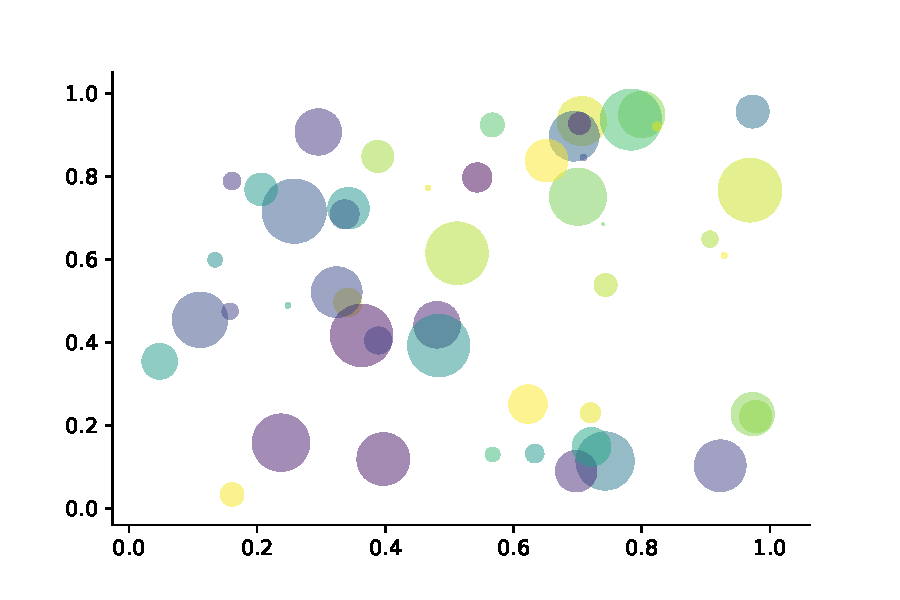
\includegraphics[width=0.6\textwidth]{scatter.pdf}
	\caption{散点图示例 $\hat{y}=a+bx$ \label{fig:scatter}}
\end{figure}

以最简单的一元线性模型来解释最小二乘法。什么是一元线性模型呢?监督学习中,如果预测的变量是离散的,我们称其为分类(如决策树,支持向量机等),如果预测的变量是连续的,我们称其为回归。回归分析中,如果只包括一个自变量和一个因变量,且二者的关系可用一条直线近似表示,这种回归分析称为一元线性回归分析。如果回归分析中包括两个或两个以上的自变量,且因变量和自变量之间是线性关系,则称为多元线性回归分析。对于二维空间线性是一条直线;对于三维空间线性是一个平面,对于多维空间线性是一个超平面。

\begin{property}
柯西列的性质
\begin{enumerate}
\item $\{x_k\}$ 是柯西列,则其子列 $\{x_k^i\}$ 也是柯西列。
\item $x_k\in \mathcal{R}^n$,$\rho(x,y)$ 是欧几里得空间,则柯西列收敛,$(\mathcal{R}^n,\rho)$ 空间是完备的。
\end{enumerate}
\end{property}

\begin{conclusion}
回归分析(regression analysis) 是确定两种或两种以上变量间相互依赖的定量关系的一种统计分析方法。运用十分广泛,回归分析按照涉及的变量的多少,分为一元回归和多元回归分析;按照因变量的多少,可分为简单回归分析和多重回归分析;按照自变量和因变量之间的关系类型,可分为线性回归分析和非线性回归分析。
\end{conclusion}

\nocite{EINAV2010,Havrylchyk2018} 

\bibliography{reference}

\appendix
\chapter{基本数学工具}

本附录包括了计量经济学中用到的一些基本数学,我们扼要论述了求和算子的各种性质,研究了线性和某些非线性方程的性质,并复习了比例和百分数。我们还介绍了一些在应用计量经济学中常见的特殊函数,包括二次函数和自然对数,前 4 节只要求基本的代数技巧,第 5 节则对微分学进行了简要回顾;虽然要理解本书的大部分内容,微积分并非必需,但在一些章末附录和第 3 篇某些高深专题中,我们还是用到了微积分。

\section{求和算子与描述统计量}

\textbf{求和算子} 是用以表达多个数求和运算的一个缩略符号,它在统计学和计量经济学分析中扮演着重要作用。如果 $\{x_i: i=1, 2, \ldots, n\}$ 表示 $n$ 个数的一个序列,那么我们就把这 $n$ 个数的和写为:

\begin{equation}
\sum_{i=1}^n x_i \equiv x_1 + x_2 +\cdots + x_n
\end{equation}


\chapter{最小示例}

\begin{lstlisting}[frame=single]
\documentclass{elegantbook}
% title info
\title{Title}
\subtitle{Subtitle is here}
% bio info
\author{Your Name}
\institute{XXX University}
\date{\today}
% extra info
\version{1.00}
\equote{Victory won\rq t come to us unless we go to it. --- M. Moore}
\logo{logo.png}
\cover{cover.jpg}

\begin{document}

\maketitle
\tableofcontents
\mainmatter
\hypersetup{pageanchor=true}
% add preface chapter here if needed
\chapter{Example Chapter Title}
The content of chapter one.

\bibliography{reference}

\appendix
\chapter{Appendix Chapter Title}
The content of appendix 1.

\end{document}
\end{lstlisting}

\end{document}
